
\chapter{Getting Started}

\section{Installation from the CFAST Web Site}

CFAST is documented by three publications, this user's guide, a technical reference guide \cite{CFAST_Tech_Guide_7} and a model evaluation guide \cite{CFAST_Valid_Guide_7}. The technical reference guide describes the underlying physical principles, provides a comparison with other models, and includes an evaluation of the model following the guidelines of ASTM E1355 \cite{ASTM:E1355}. The model evaluation guide documents verification and validation efforts for the model. This user's guide describes how to use the model and applies to version 67 and later.  All the documentation is available on the web site.

All of the files associated with CFAST can be obtained at:

\begin{lstlisting}
http://cfast.nist.gov
\end{lstlisting}

\begin{wrapfigure}{r}{3.2in}
  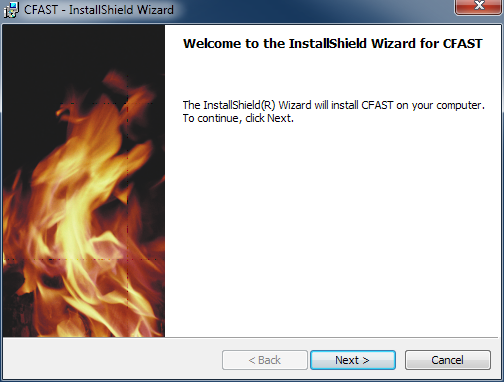
\includegraphics[width=3.1in]{FIGURES/Getting_Started/Install}
\end{wrapfigure}

Information about new versions, bug fixes, and documentation for the model and software are available on this web site.  The CFAST distribution consists of a self-extracting set-up program for Windows-based PCs.

After downloading the set-up program to a PC, double-clicking on the file's icon walks the user through a series of steps for installation of the program.  The most important part of the installation is the creation of a folder (typically c:$\backslash$Program Files$\backslash$CFAST by default) in which the CFAST executable files and supplemental data files are installed.  Sample input files are placed in a folder called Examples off this folder.

\section{Computer Hardware Requirements}
CFAST requires a relatively fast processor and a sufficient amount of random-access memory (RAM) for complex cases. Typical calculation times for a multi-compartment scenario can range from a few seconds to multiple hours, depending on the details of the scenario. Plus, hard drive storage is needed to store the output of calculations.  It is not uncommon for a single calculation to generate output files as large as several hundred megabytes.

\section{Verifying Correct Installation and Operation}
Sample input files are provided with the program for new users who are encouraged to first run the sample calculations before attempting to create an input file. To run the model, browse to the location of the CFAST sample input file (default location is in a folder called Examples off the installation folder, copy the file named standard.in to a location of your choice (for example, in a created folder of the ``My Documents'' folder and then double click on the copied file.  This should open the file in the CFAST input editor, CEdit.  The simple test case can be run from the program menu by selecting 'Run!' and then 'Model Simulation, CFAST'

This runs a very simple test case and it should be completed quickly. Additional details on running CFAST are included in the next chapter. To verify that the installation has been done correctly, the output of the model should appear as follows.

\begin{figure}[h!]
\begin{center}
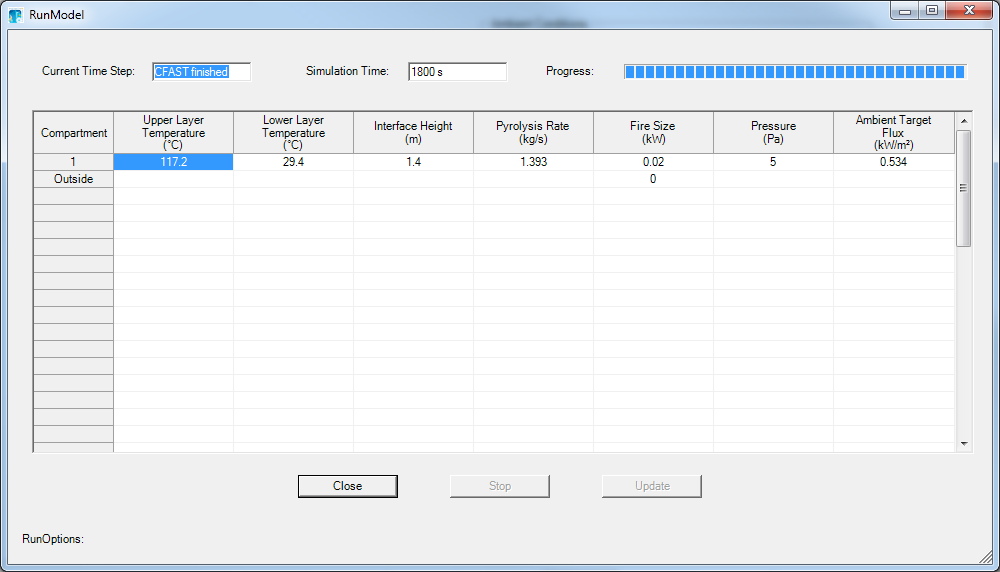
\includegraphics[width=6.5in]{FIGURES/Getting_Started/Standard_Output}
\end{center}
\end{figure}

This case checks several attributes of the installation to insure the software is running correctly. Additional explanation of the results of this run is described in Chapter 5.
